% !TeX root = index.tex
\iffalse
This chapter lays out your approach. 
What did you actually do to reach your goal, or attempt to reach your goal? 
What equipment did you use? 
How did you build the device? 
How did you set up the simulation: what mesh values, for example, did you use?

Provide enough detail that your work can be duplicated by someone else.
Be precise and use the correct units.
\fi


This section describes methods and design choices used to construct RISC and OISC processors.

\subsection{Machine Code}\label{subsec:machine_code}
Machine code subsection talks about instructions and how they are encoded.

\subsubsection{RISC Machine Code}
One of the aim is to ensure instruction size is to be as minimal. An 8bit instruction width was chosen with an optional additional immediate value from one to three bytes. Immediate value operation is expanded upon in section \ref{subsec:imm_values}.

The decision was made to have an instruction to composed of operation code and two operands — first source \& destination and second only source. This is more similar to x86 architecture rather than to MIPS. Three possible combinations of register address sizes are possible, from one to three bits in order to fit them in a single instruction. Two bits was the chosen option as it allows the addressing of four general purpose registers which is sufficient for most applications, and allowed four bits for operation code — allowing up to 16 instructions. 

Due to a small amount of possible operation codes and not all instructions requiring operate with two operands (for example, \texttt{JUMP} instruction does not need any operands, set immediate value only needs one operand), other two type instructions are added to the design — with one and zero operands. See figure \ref{fig:risc_machinecode}. This enables the processor to have 45 different instructions while maintaining minimal instruction size. Final design has:
\begin{description}[labelindent=1cm, labelsep=1em]
	\item[$\bullet$ \textbf{8 }]  2-operand instructions
	\item[$\bullet$ \textbf{32}]  1-operand instructions
	\item[$\bullet$ \textbf{5 }]  0-operand instructions
\end{description}
Full list of RISC instructions is listed in Table \ref{tab:risc_instructions} in an \nameref{sec:appendix} section.

\begin{blockpage}
\begin{gather*}
\scalebox{0.8}{2 operands:}~
\underbrace{
	\colorbox{c1}{0}\,
	\colorbox{c1}{1}\,
	\colorbox{c1}{2}\,
	\colorbox{c1}{3}
}_\text{op. code}
\underbrace{
	\colorbox{c2}{4}\,
	\colorbox{c2}{5}
}_\text{dst.}
\underbrace{
	\colorbox{c3}{6}\,
	\colorbox{c3}{7}
}_\text{src.}
\\
\scalebox{0.8}{1 operand:}~
\underbrace{
	\colorbox{c1}{0}\,
	\colorbox{c1}{1}\,
	\colorbox{c1}{2}\,
	\colorbox{c1}{3}
}_\text{op. code}
\underbrace{
	\colorbox{c2}{4}\,
	\colorbox{c2}{5}
}_\text{dst.}
\underbrace{
	\colorbox{c1}{6}\,
	\colorbox{c1}{7}
}_\text{op. c.}\\
\scalebox{0.8}{0 operands:}~
\underbrace{
	\colorbox{c1}{0}\,
	\colorbox{c1}{1}\,
	\colorbox{c1}{2}\,
	\colorbox{c1}{3}\,
	\colorbox{c1}{4}\,
	\colorbox{c1}{5}\,
	\colorbox{c1}{6}\,
	\colorbox{c1}{7}
}_\text{operation code}
\end{gather*}
\begin{center}
\captionof{figure}{\textit{RISC instructions composition. Number inside box represents bit index. Destination (dst.) bits represents of source and destination register address.}}
\label{fig:risc_machinecode}
\end{center}
\end{blockpage}

\subsubsection{OISC Machine Code}

As OISC operaten on a single instruction, the composition of each instruction mainly consists of two parts — source and destination. In order to allow higher instruction flexibility, an immediate flag has been added which sets source address to represent an immediate value. The composition of finalised machine code is shown in figure \ref{fig:oisc_machinecode}. 

\begin{blockpage}
\begin{gather*}
\underbrace{
	\colorbox{c1}{0}
}_\text{imm.}
\underbrace{
	\colorbox{c2}{1}\,
	\colorbox{c2}{2}\,
	\colorbox{c2}{3}\,
	\colorbox{c2}{4}\,
}_\text{destination}
\underbrace{
	\colorbox{c3}{5}\,
	\colorbox{c3}{6}\,
	\colorbox{c3}{7}\,
	\colorbox{c3}{8}\,
	\colorbox{c3}{9}\,
	\colorbox{c3}{10}\,
	\colorbox{c3}{11}\,
	\colorbox{c3}{12}
}_\text{source}
\end{gather*}

\begin{center}
\captionof{figure}{\textit{OISC instruction composition. Number inside box represents bit index.}}
\label{fig:oisc_machinecode}
\end{center}
\end{blockpage}

The decision was made for source address to be 8bits, to match an immediate value and data bus width. The destination address was chosen to be as minimal as possible, leaving only four bits and 16 executable destinations. The final design has \textbf{15} destination and \textbf{41} source addresses. This is not the most space efficient design as 41 source addresses could be implemented with only six bits, not using two bits every time a non-immediate source is used.

A comprehensive list of OISC sources and destinations are given in Table \ref{tab:oisc_instructions} in an \nameref{sec:appendix} section.

\begin{landscape}
	\subsection{Data flow} \label{sec:dataflow}
	\subsubsection{RISC Datapath} \label{subsec:datapath}
	\begin{figure}[h!]
		\centering
		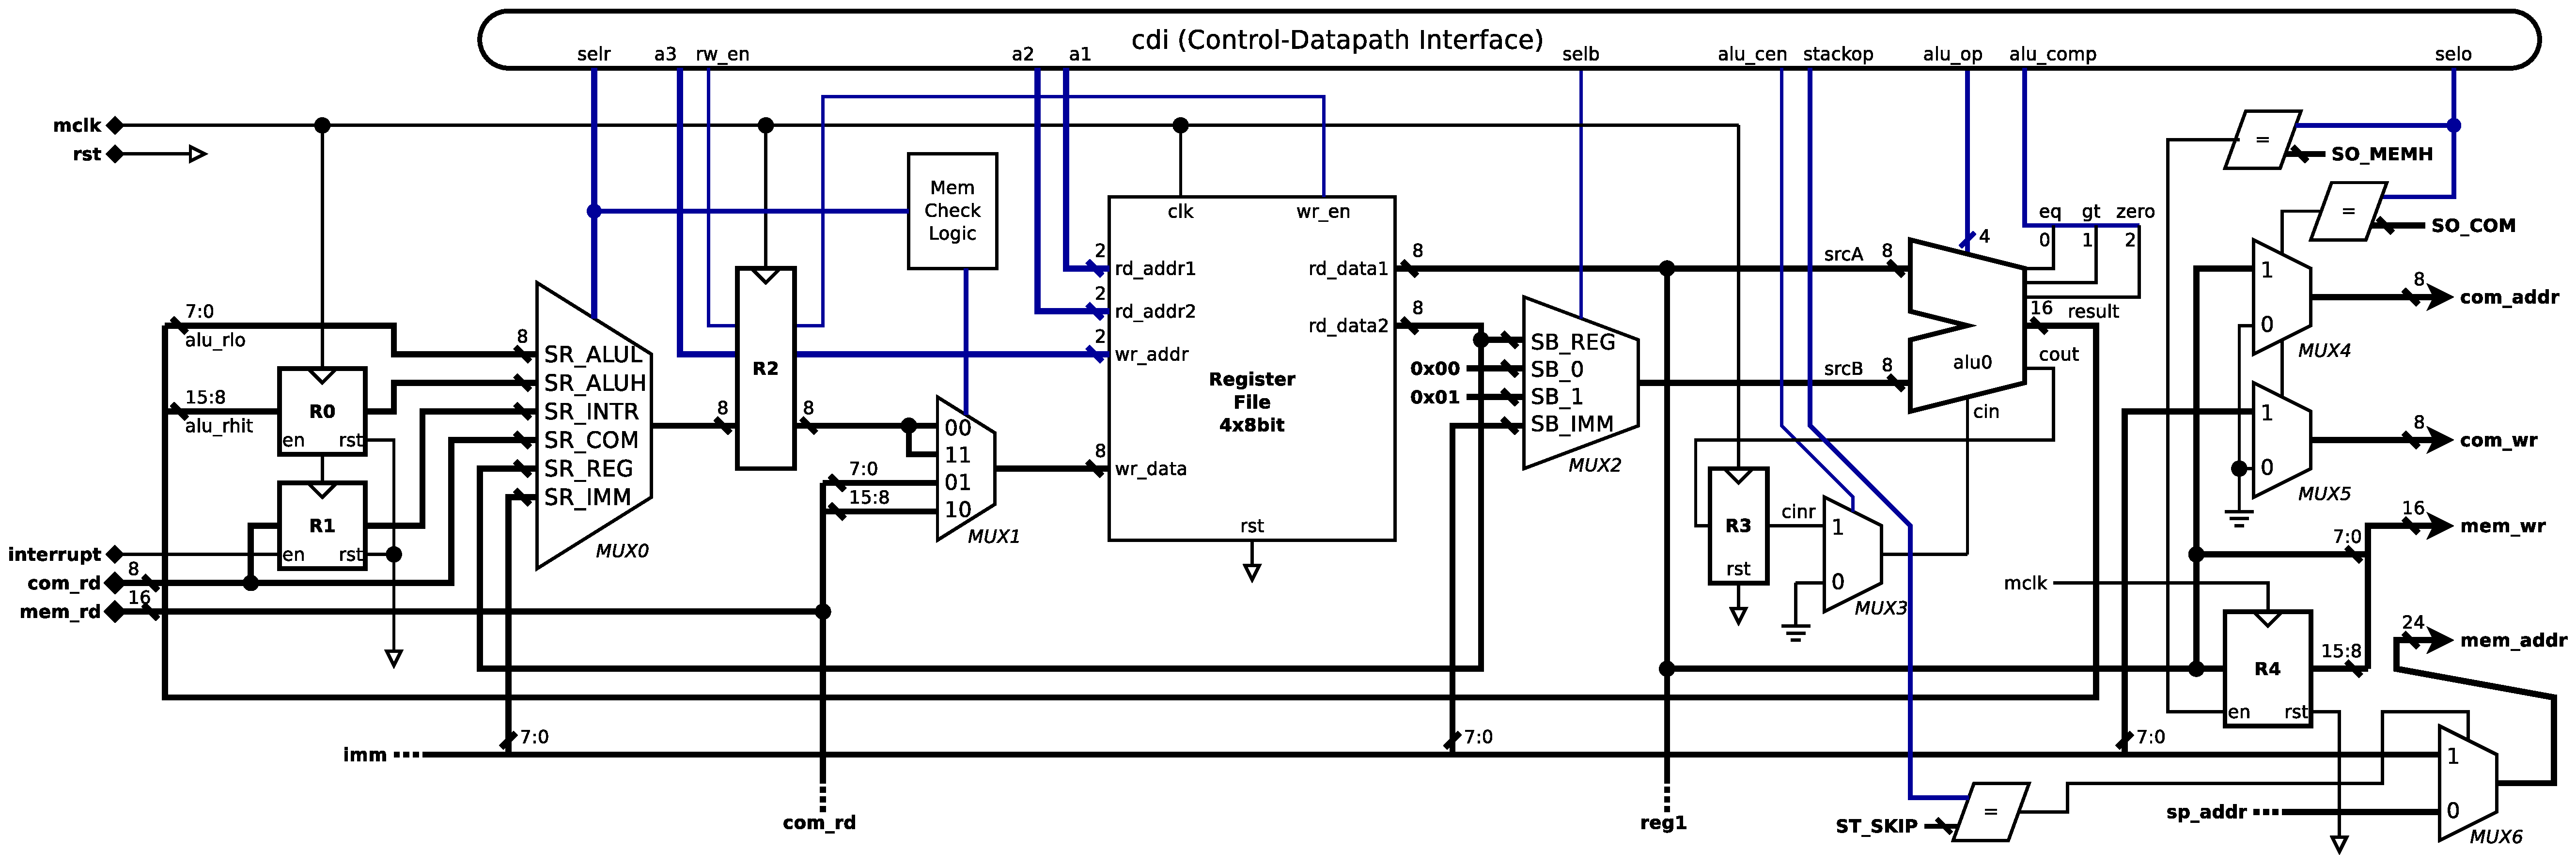
\includegraphics[width=\linewidth]{../resources/datapath.eps}
		\caption{Digital diagram of RISC datapath}
		\label{fig:datapath}	
	\end{figure}
	
	Figure \ref{fig:datapath} above represents a partial RISC datapath. This diagram can be extended to Program counter, Stack pointer and Immediate Override logics are shown in figures \ref{fig:risc_pc}, \ref{fig:risc_stack} and \ref{fig:risc_imo} respectively. CDI (Control-Data Interface) is a HDL (Hardware Description Language) concept that connect datapath and control unit together. The immediate value is provided to datapath by IMO block described in section \ref{subsec:imo}.\\
	Data to register file is selected and saved with \textit{MUX0}. This data is delayed by one cycle with \textit{R2} to match timing that of data taken from the memory. If \texttt{LWLO} or \texttt{LWHI} instructions are executed, \textit{MUX1} select high or low byte from memory to read. In order to compensate for timing, as value written to register file is delayed by one cycle, register file has internal logic that outputs \textit{wr\_data} to \textit{rd\_data1} or/and  \textit{rd\_data2} immediately if \textit{wr\_en} is high and \textit{rd\_addr1} or/and \textit{rd\_addr2} matches \textit{wr\_addr}, making it act more like latch. \\
\end{landscape}
\textit{MUX2}allows to override ALU source B, \textit{R3} and \textit{MUX3} enables control unit to enable ALU carry in bit, allowing multi-word number addition/subtraction. \textit{MUX4} and \textit{MUX5} allows sending data to the COM block with \texttt{COM} instruction. If any other instruction performed, then \textit{0x00} byte for COM address and data is sent, indicating no action. Data can be stored to memory only with a \texttt{SWLO} instruction. It writes high byte value whatever is stored in \textit{R4} register. This buffer can be written to using a \texttt{SWHI} instruction. Therefore, to change only a single byte in a particular memory location, other byte has to be fetched in advanced and used in a \texttt{SWLO} or \texttt{SWHI} instruction. \textit{MUX6} selects memory address value from the \textit{imm} or stack pointer.

\subsubsection{OISC Datapath} \label{subsec:oisc_cells}
OISC datapath only consists of instruction-data bus and a small circuit that connect them to logic blocks that computes the data. These logic blocks can represent ALU operation combinational logic, or any other part of a processor as shown in Figure \ref{fig:oisc_simple}.

Figure \ref{fig:oisc_cell_in} represents a common destination circuit. It checks if a particular logic block destination address matches one in instruction bus, then enables latch and also sets flag that destination is used to the further logic. 
\begin{colfigure}
	\centering
	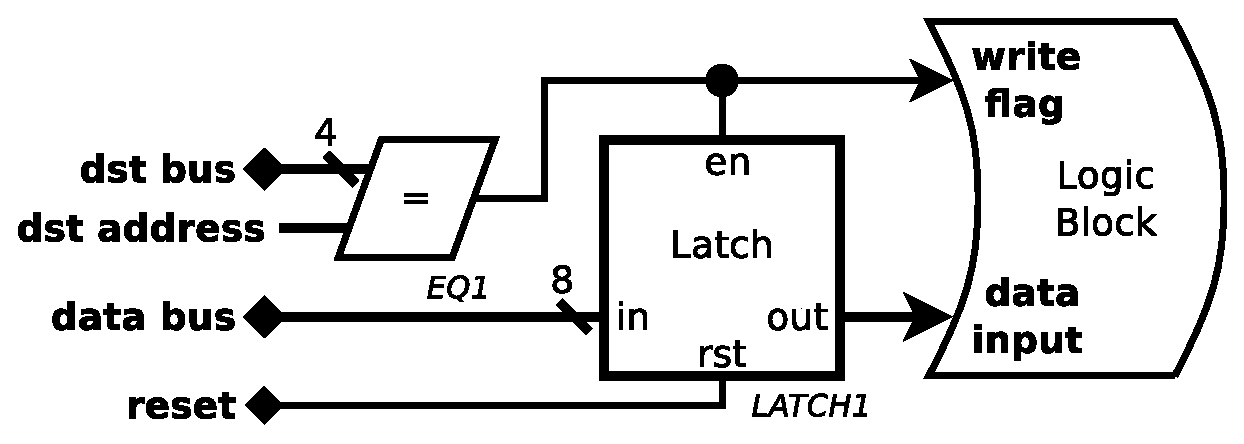
\includegraphics[width=\linewidth]{../resources/oisc_cell_in.eps}
	\captionof{figure}{OISC processor data bus to destination connection logic}
	\label{fig:oisc_cell_in}
\end{colfigure}

Similarly, Figure \ref{fig:oisc_cell_out} represents a source circuit connecting output of a logic block. Logic block can be assumed to only contain combinational logic, therefore a register is placed at the output of it. A buffer \textit{BUF1} is used to connect data in a register \textit{REG1} to the data bus. This ensures that only one bus driver is present, ensuring no data collision. 

\begin{colfigure}
	\centering
	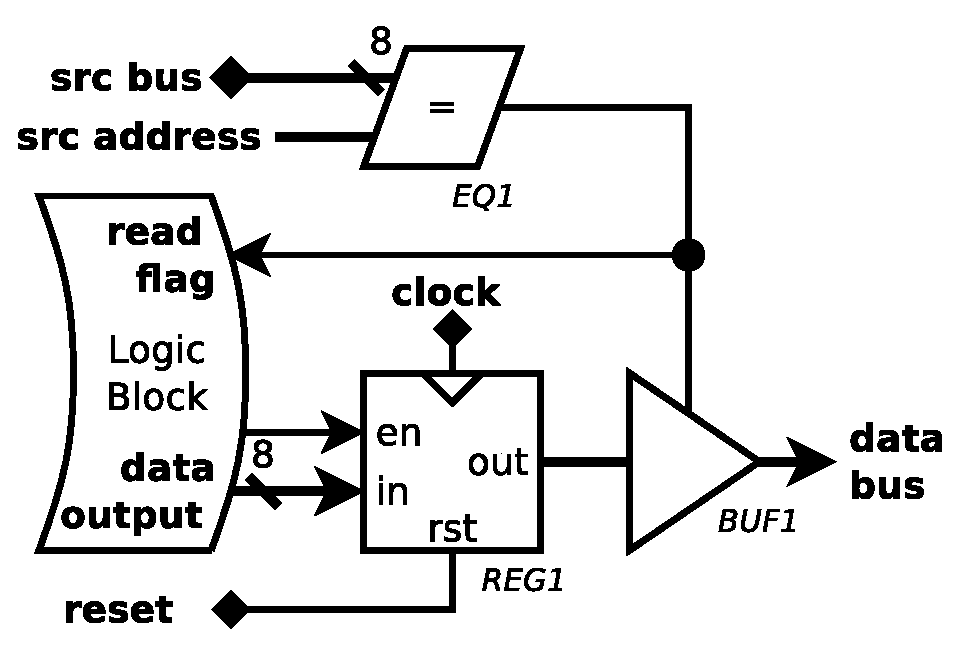
\includegraphics[width=\linewidth]{../resources/oisc_cell_out.eps}
	\captionof{figure}{OISC processor data bus to source connection logic}
	\label{fig:oisc_cell_out}
\end{colfigure}

The general timing is designed so that the information at the source is immediately ready on the data bus at rise of the processor clock. The source is connected to the destination connection where combinational logic is present. 

\subsubsection{OISC Datapath Implementation Problems} \label{subsec:oisc_cell_issue}

The complete implementation using latches for destination logic was not successful. Latches did not operate correctly when synthesised onto FPGA. This issue might be caused by some timing problem between some combination of source and destination logic. The exact cause was not resolved.

As a quick solution, latches at the destination have been replaced with a clocked register that is triggered at negative clock edge, which is opposite to source register trigger. This solution has resolved issue, however it effectively reduces the period of time that data has to propagate though logic blocks between source and destination by two.

\subsection{Stack} \label{subsec:stack}
This section describes dedicated logic for stack pointer control at both processors. The stack pointer starts from the highest memory address value and "stacks" towards lower address values. Both designs were simplified to only operate on two byte addresses, meaning that stack pointer has a constant \texttt{FFh} value at the least significant byte.


\subsubsection{RISC Stack}
The RISC processor implements the stack pointer that is used in \texttt{PUSH}, \texttt{POP}, \texttt{CALL} and \texttt{RET} instructions. Figure \ref{fig:risc_stack} represents the logic diagram for stack pointer. This circuit also supports \textit{pc\_halted} signal from the program counter to prevent the stack pointer from being added by 1 twice during the \texttt{RET} instruction. 

One of the problems with the current stack pointer implementation is 8bit data stored in 16bit memory address, wasting a byte, except when storing the program pointer with \texttt{CALL} instruction. This can be improved by adding a high byte register, however then it would cause complications when a 16bit program pointer is stored with \texttt{CALL} instruction. This can still be improved with a more complex circuit, or by using memory cache with 8bit data input. However, with the current implementation this does not affect processor comparison, it only increases stack size in memory.

\begin{figure*}
	\centering
	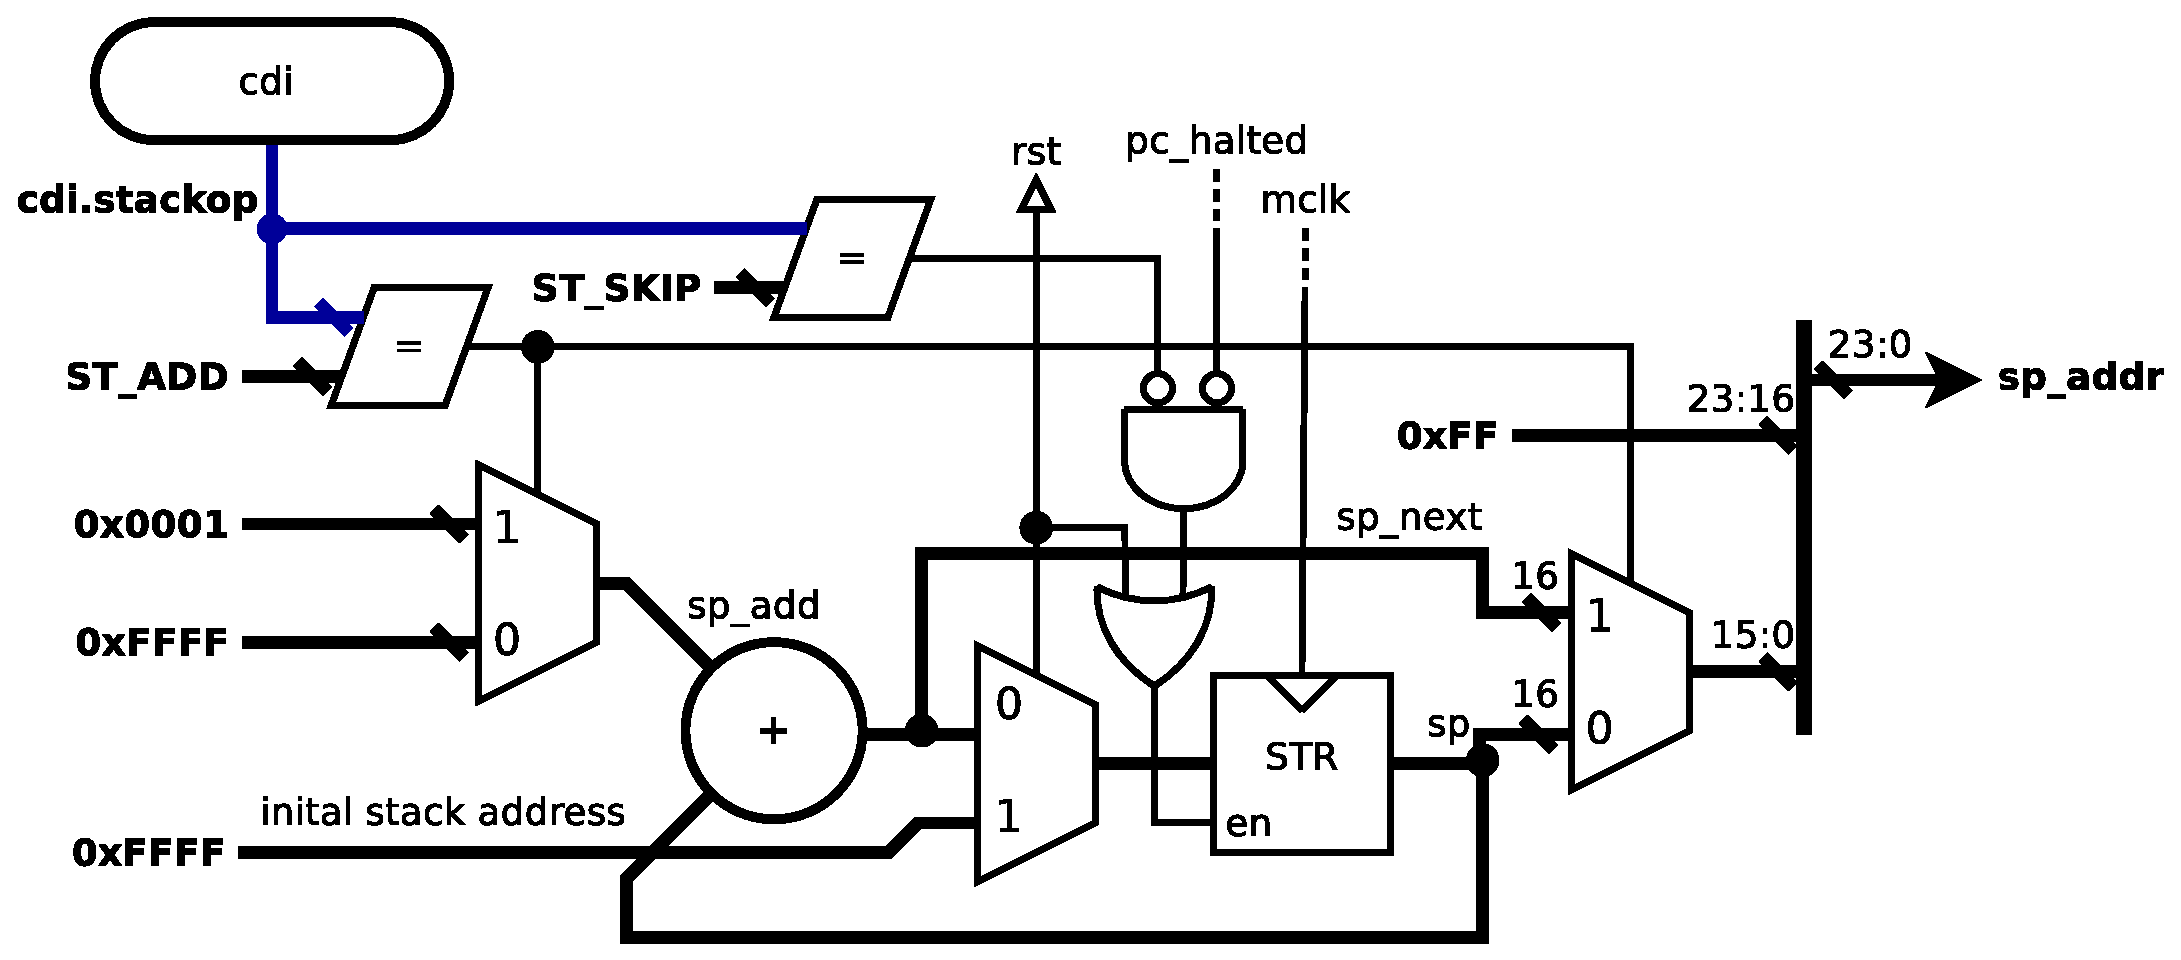
\includegraphics[scale=0.4]{../resources/risc_stack.eps}
	\caption{Digital diagram of RISC stack pointer logic}
	\label{fig:risc_stack}
\end{figure*}

\subsubsection{OISC Stack}

The stack pointer circuit in OISC is very similar to RISC. When reset, push or pop flags are set, it changes the state of stack pointer by adding or subtracting its value by one, or resetting it to default. Logic diagram is shown in Figure \ref{fig:oisc_stack}.
\begin{figure*}[b]
	\centering
	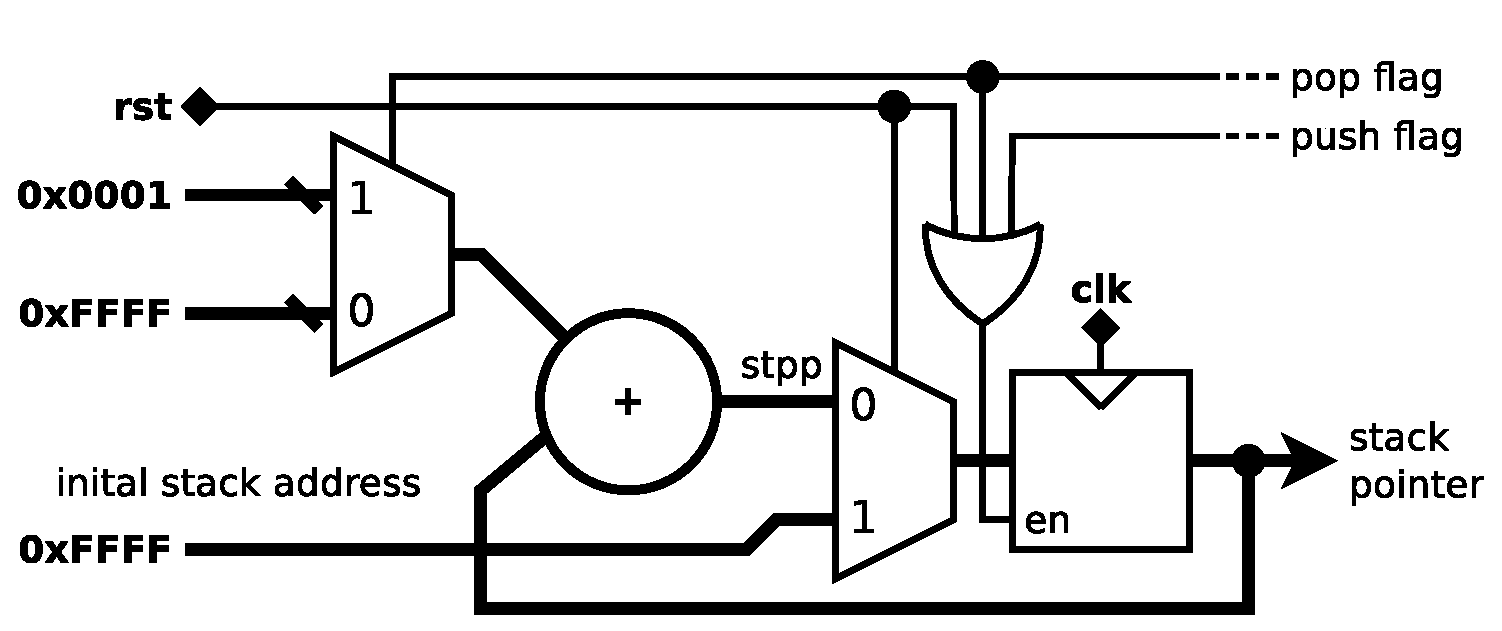
\includegraphics[scale=0.4]{../resources/oisc_stack.eps}
	\caption{Digital diagram of OISC stack pointer logic}
	\label{fig:oisc_stack}
\end{figure*}

Logic diagram of stack control unique to OISC processor is shown in Figure \ref{fig:oisc_stack_2}. Push and pop flags are taken from the source and destination logic. A cached value of last stored value is kept, so that it would be immediately available on source request. Pop flag is delayed by one clock cycle. This ensures that once stack value is popped, lower stack value is written into the cache during next the clock cycle. Note that there is an issue with this design, stack source or destination instruction cannot be used together with other stack or memory operations as it creates a collision accessing system memory at the same time. This collision can be avoided with software however. 
\begin{figure*}
	\centering
	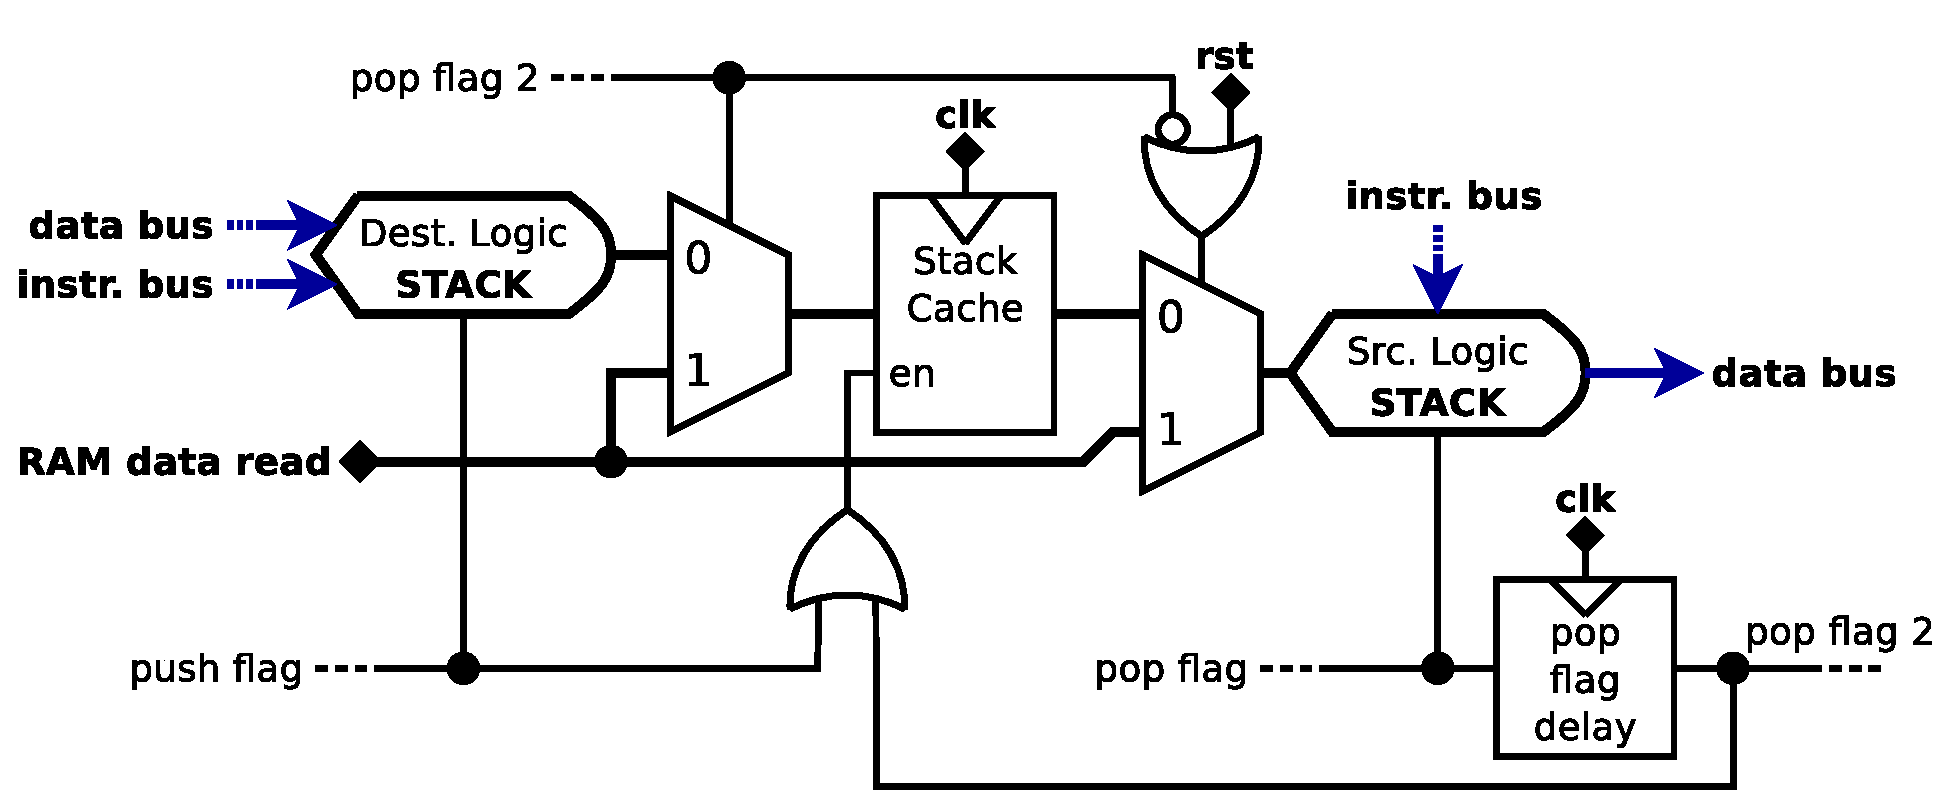
\includegraphics[scale=0.4]{../resources/oisc_stack_2.eps}
	\caption{Digital diagram of OISC stack control logic}
	\label{fig:oisc_stack_2}
\end{figure*}

\subsection{Program Counters} \label{subsec:pc}
In this subsection, program counter and their differences will be described.

\subsubsection{RISC Program Counter}

\begin{figure*}[h!]
	\centering
	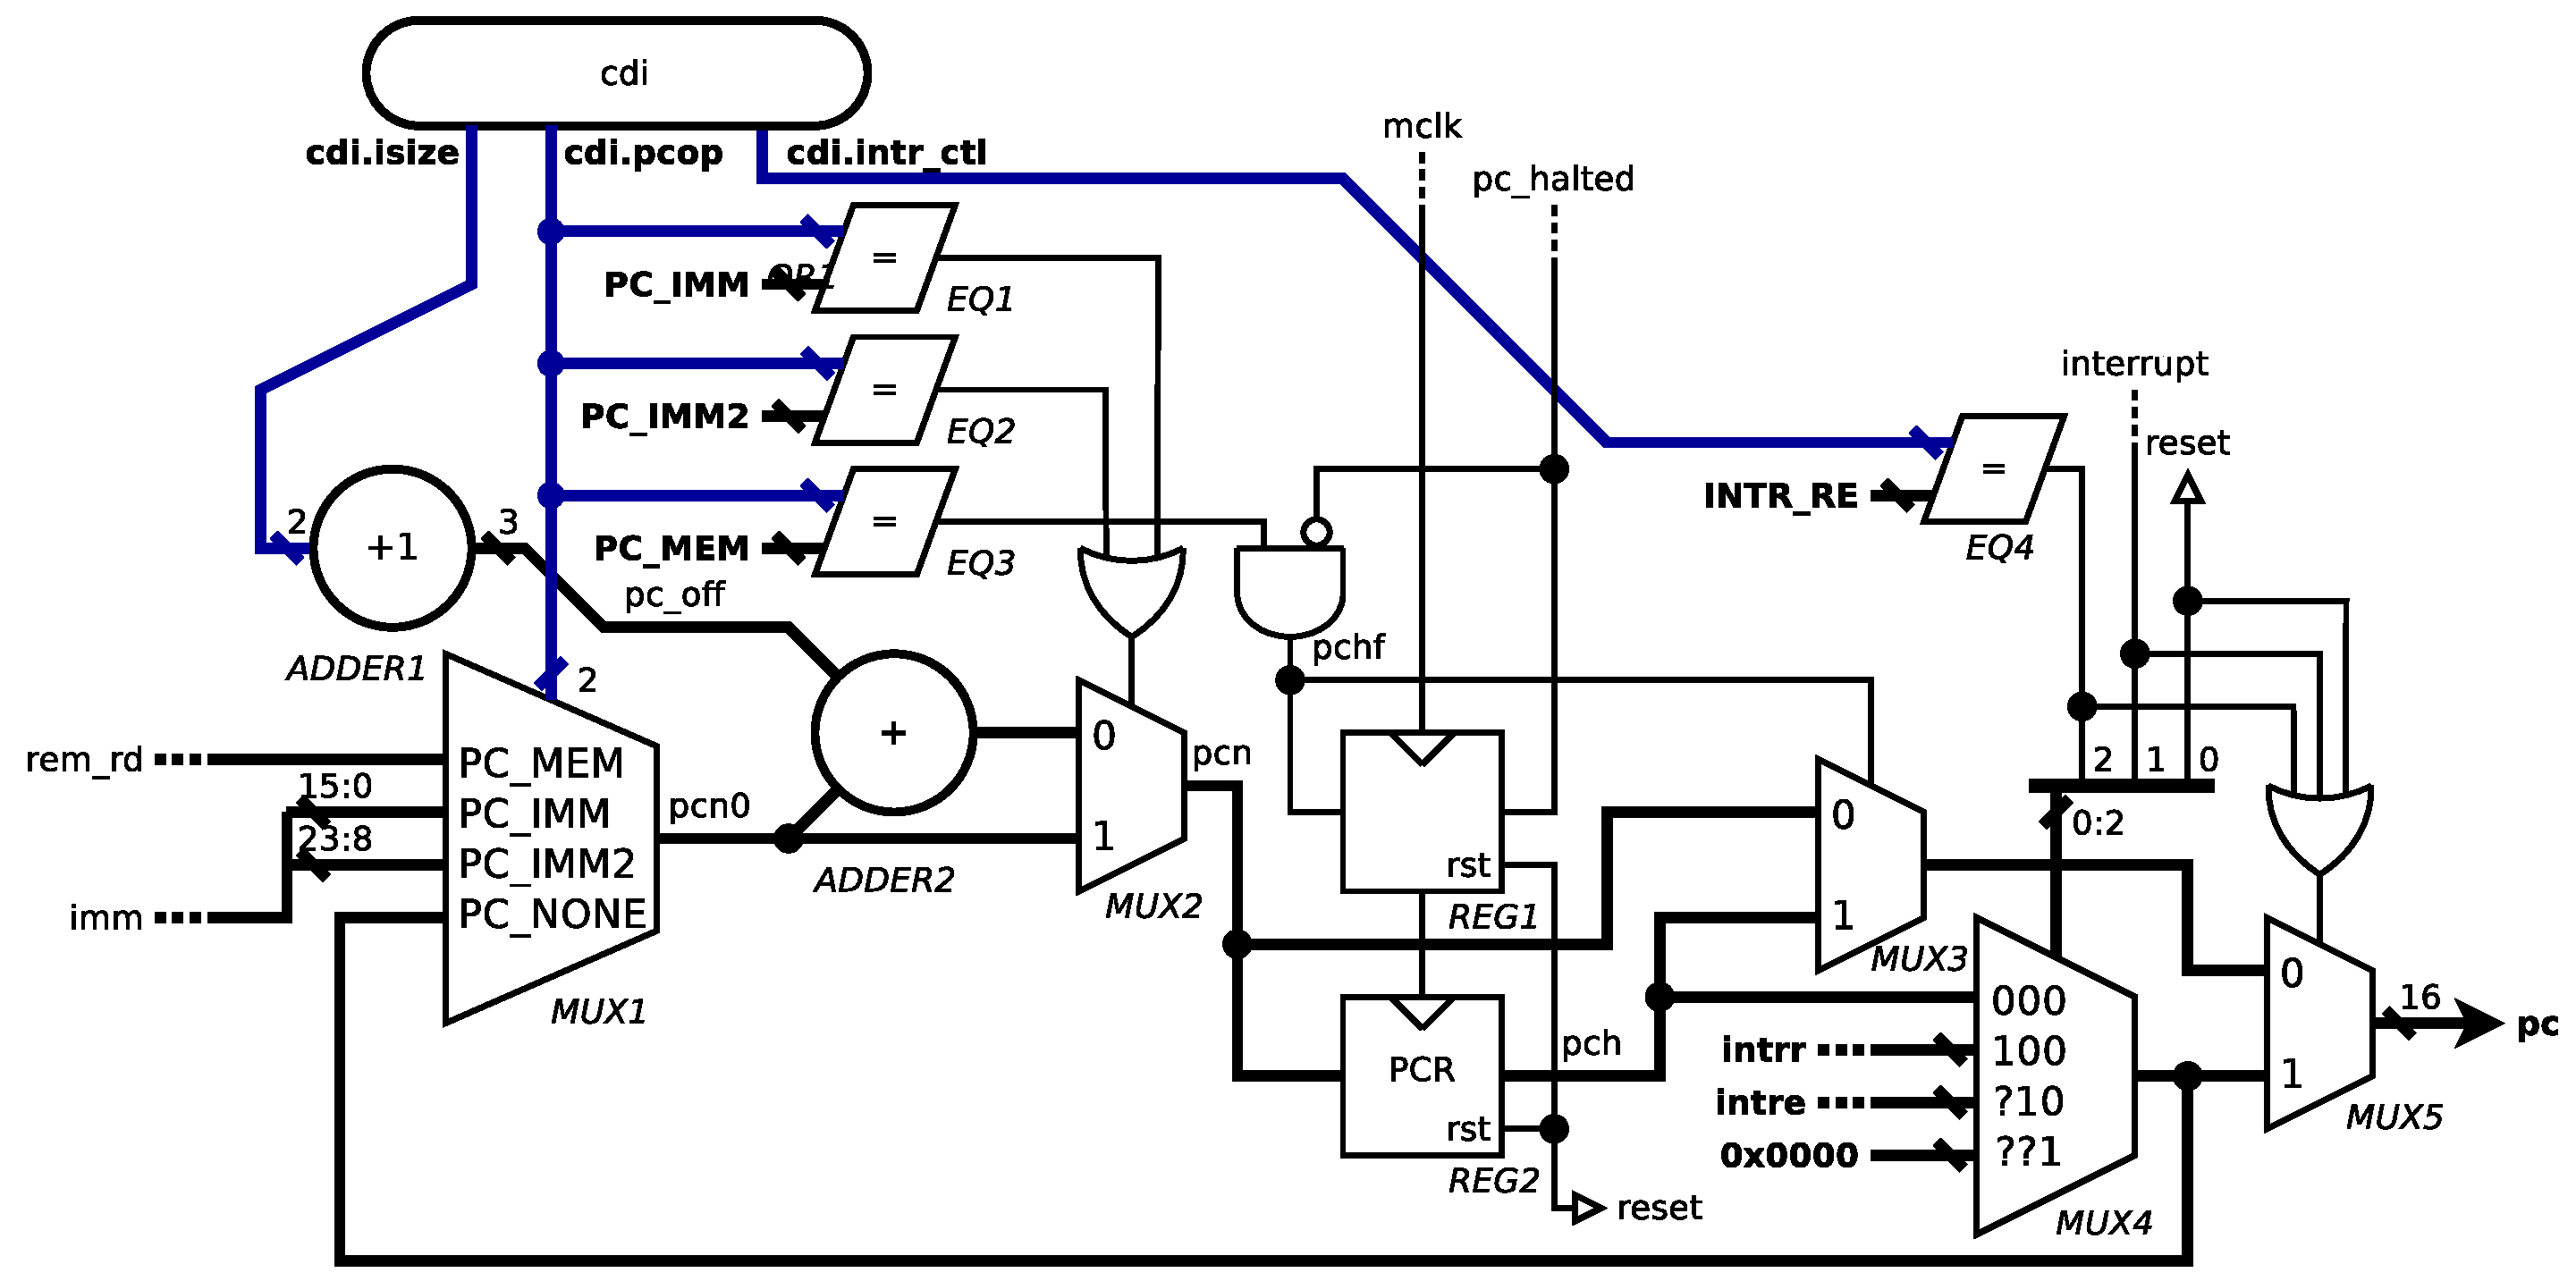
\includegraphics[width=\linewidth]{../resources/risc_pc.eps}
	\caption{Digital diagram of RISC program counter}
	\label{fig:risc_pc}
\end{figure*}

Figure \ref{fig:risc_pc} represents the digital diagram for a program counter. There are a few key features about this design: it can take values from memory for \texttt{RET} instruction; immediate value (\textit{PC\_IMM2} is shifted by one byte to allow \texttt{BEQ}, \texttt{BGT}, \texttt{BGE} instructions as first immediate byte used as ALU source B); it can jump to an interrupt address; it produces a \textit{pc\_halted} signal when memory is read (\texttt{RET} instruction takes two cycles, because cycle one fetches the address from stack and second cycle fetches the instruction from the instruction memory).

\subsubsection{OISC Program Counter}\label{subsec:oisc_pc}
 
OISC program counter is much simpler than RISC, as it does not have variable length instruction, delay flags for \texttt{RET} operation, or logic for selecting branch source address. 
 
\begin{colfigure}
	\centering
	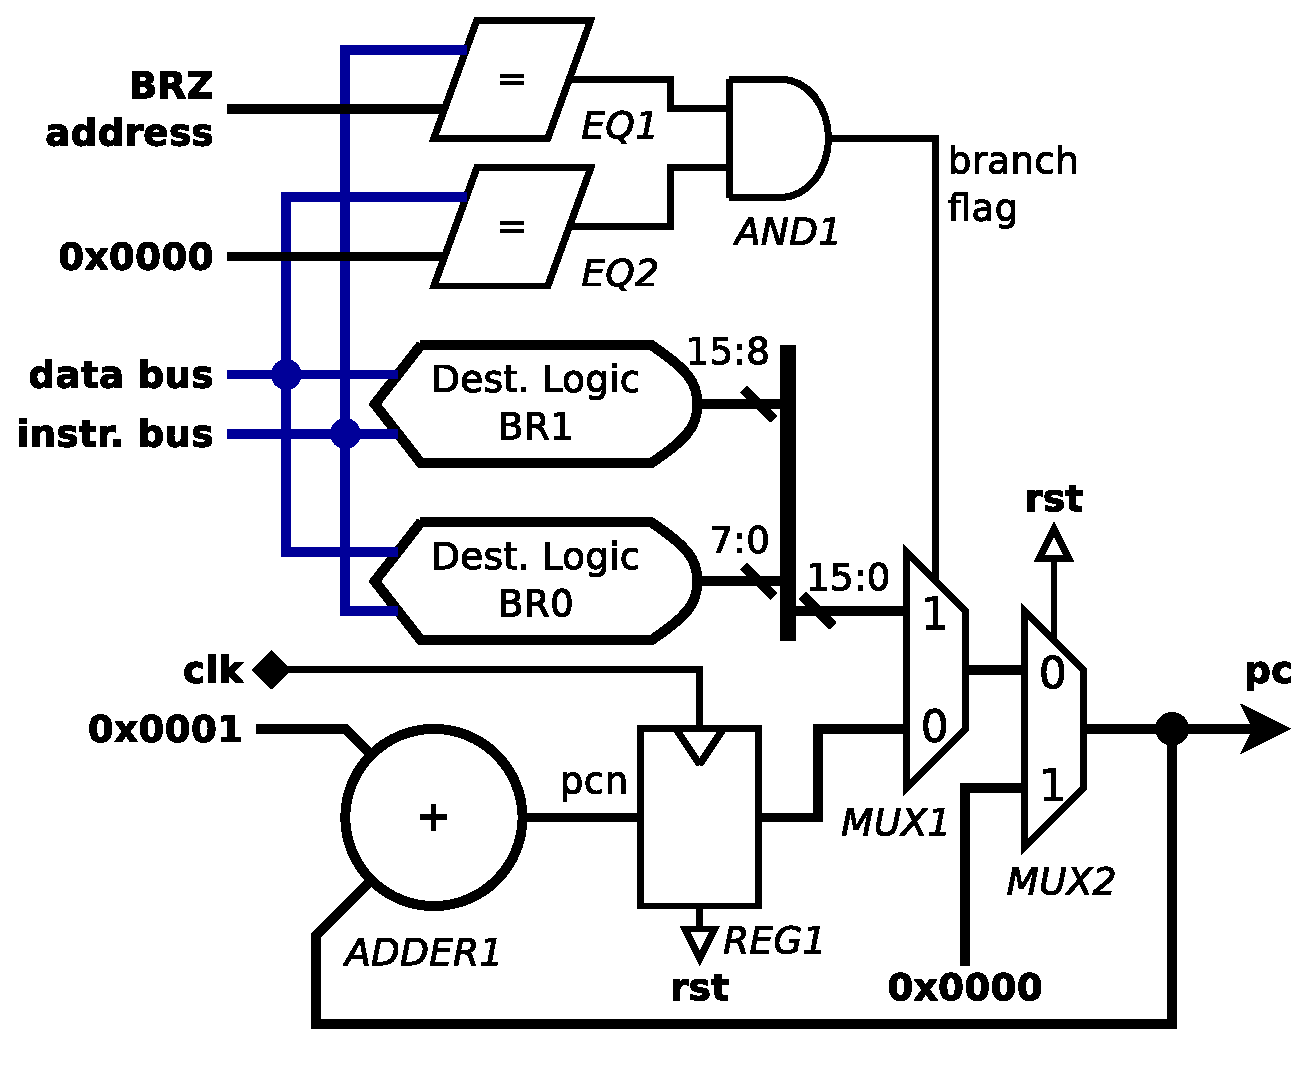
\includegraphics[width=\linewidth]{../resources/oisc_pc.eps}
	\captionof{figure}{Digital diagram of OISC program counter}
	\label{fig:oisc_pc}
\end{colfigure}

Looking at Figure \ref{fig:oisc_pc} bottom, the basic operation is to just add one to previous program counter with \textit{ADDER1} and \textit{REG1}, reset it to zero at reset with \textit{MUX2}. Two destination logic blocks are used as accumulators to store branch address. Once an instruction with the \texttt{BRZ} destination is executed, comparator \textit{EQ2} checks if the data bus value is equal to zero. If this condition is met, it enables \textit{MUX1} and overrides program counter to address stored in \texttt{BR0} and \texttt{BR1} accumulators. Unlike in RISC however, it requires three instructions to set new address and jump. Similarly, \texttt{CALL} and \texttt{RET} requires five and three instructions respectively. RISC equivalent instructions are show in Listing \ref{code:oisc_jump}.

\begin{blockpage}
	\begin{lstlisting}[frame=single, emph={JUMP, CALL, RET, return}, label=code:oisc_jump, caption={OISC assembly code emulating RISC \texttt{JUMP}, \texttt{CALL} and \texttt{RET} instructions.}]
%macro JUMP 1
  BR1 %1 @1
  BR0 %1 @0
  BRZ 0x00
%endmacro

%macro CALL 1
  BR1 %1 @1
  BR0 %1 @0
  STACK %%return @1
  STACK %%return @0
  BRZ 0x00
  %%return:
%endmacro

%macro RET 0
  BR0 STACK
  BR1 STACK
  BRZ 0x00
%endmacro
	\end{lstlisting}
\end{blockpage}

\subsection{Arithmetic Logic Unit}\label{subsec:alu}

\begin{figure*}[b]
\centering
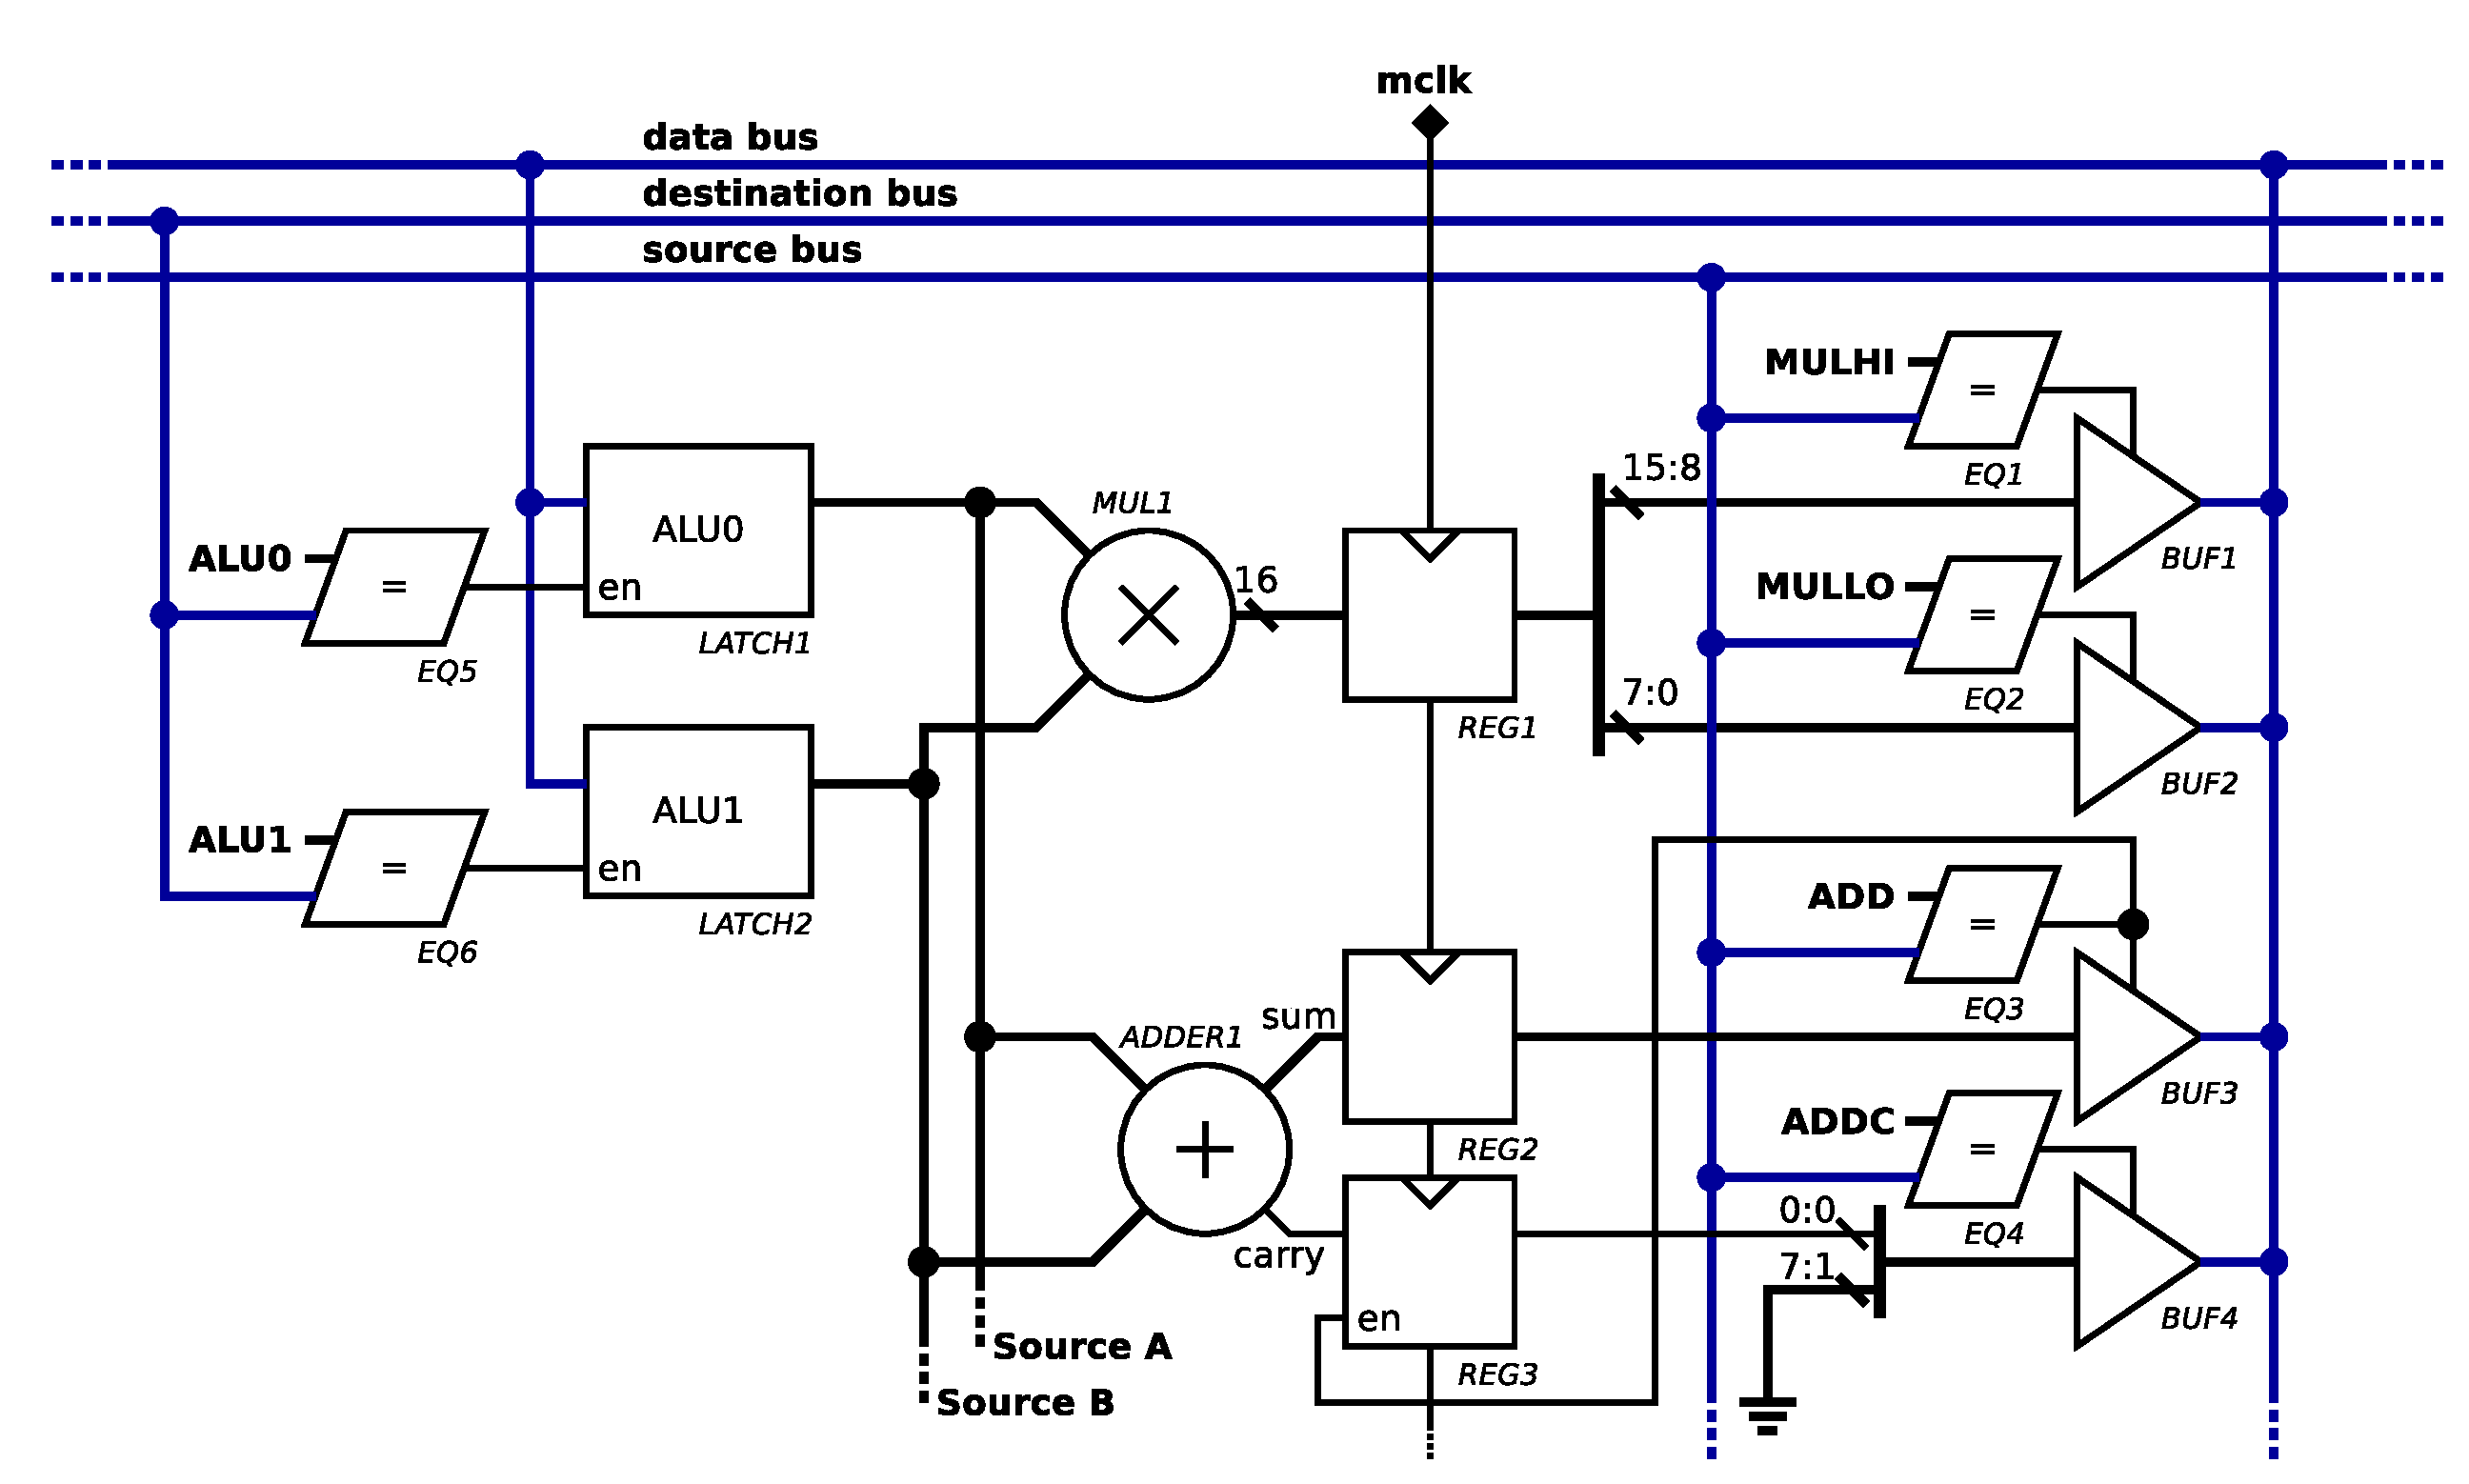
\includegraphics[scale=0.35]{../resources/oisc_alu.eps}
\caption{Digital diagram of OISC partial ALU logic}
\label{fig:oisc_alu}
\end{figure*}

This section will discuss ALU implementations of both processors. For fair comparison between OISC and RISC, ALU in both system will have the same capabilities as described in Table \ref{tab:alu_set}.

\begin{blockpage}
	\arrayrulecolor{black}
	\begin{tabular}{| c | p{0.75\linewidth} |} \hline 
		\rowcolor[rgb]{0.82,0.82,0.82}
		Name & Description \\\hline
		\arrayrulecolor[rgb]{0.82,0.82,0.82}
		ADD & Arithmetic addition (inc. carry) \\\hline
		SUB & Arithmetic subtraction (inc. carry) \\\hline
		AND & Bitwise AND \\\hline
		OR  & Bitwise OR \\\hline
		XOR & Bitwise XOR \\\hline
		SLL & Shift left logical \\\hline
		SRL & Shift right logical \\\hline
		ROL & Shifted carry from previous SLL \\\hline
		ROR & Shifted carry from previous SRL \\\hline
		MUL & Arithmetic multiplication \\\hline
		DIV & Arithmetic division \\\hline
		MOD & Arithmetic modulo \\
		\arrayrulecolor[rgb]{0,0,0}\hline
	\end{tabular}
	\captionof{table}{\textit{Supported ALU commands for both processors}}
	\label{tab:alu_set}
\end{blockpage}

\subsubsection{OISC ALU}
Due to the structure of the OISC processor, ALU source A and B are two latches that are written into when \texttt{ALU0} or \texttt{ALU1} destination address is present. ALU sources are connected with every ALU operator and performed in single clock cycle. This value is stored in a register so that it would be immediately available in a next clock cycle as a source data, as explained in \nameref{subsec:oisc_cells} Section. Figure \ref{fig:oisc_alu} represents a logic diagram of ALU with only an addition and multiplication operations present. Note that the output of \textit{EQ3} is connected to enable of \textit{REG3}, enabling output of carry to be only read after \texttt{ADD} source is requested. Similar configuration is also used for \texttt{SUB}, \texttt{ROL} and \texttt{ROR} operations.

\subsubsection{RISC ALU}
The RISC processor has very similar structure to OISC, however with two exceptions. Inputs to ALU comes from datapath data router logic. Output buffers are replaced by one multiplexer that selects a single output from all ALU operations. Another point is that RISC ALU output is 16bit, higher byte saved in "ALU high byte register" for \texttt{MUL}, \texttt{MOD}, \texttt{ROL} and \texttt{ROR} operations. This register is accessible with \texttt{GETAH} instruction.

\subsection{Program Memory}\label{subsec:memory}
This section describes how instruction memory (ROM) is implemented for both processors.

\begin{figure*}[b]
	\centering
	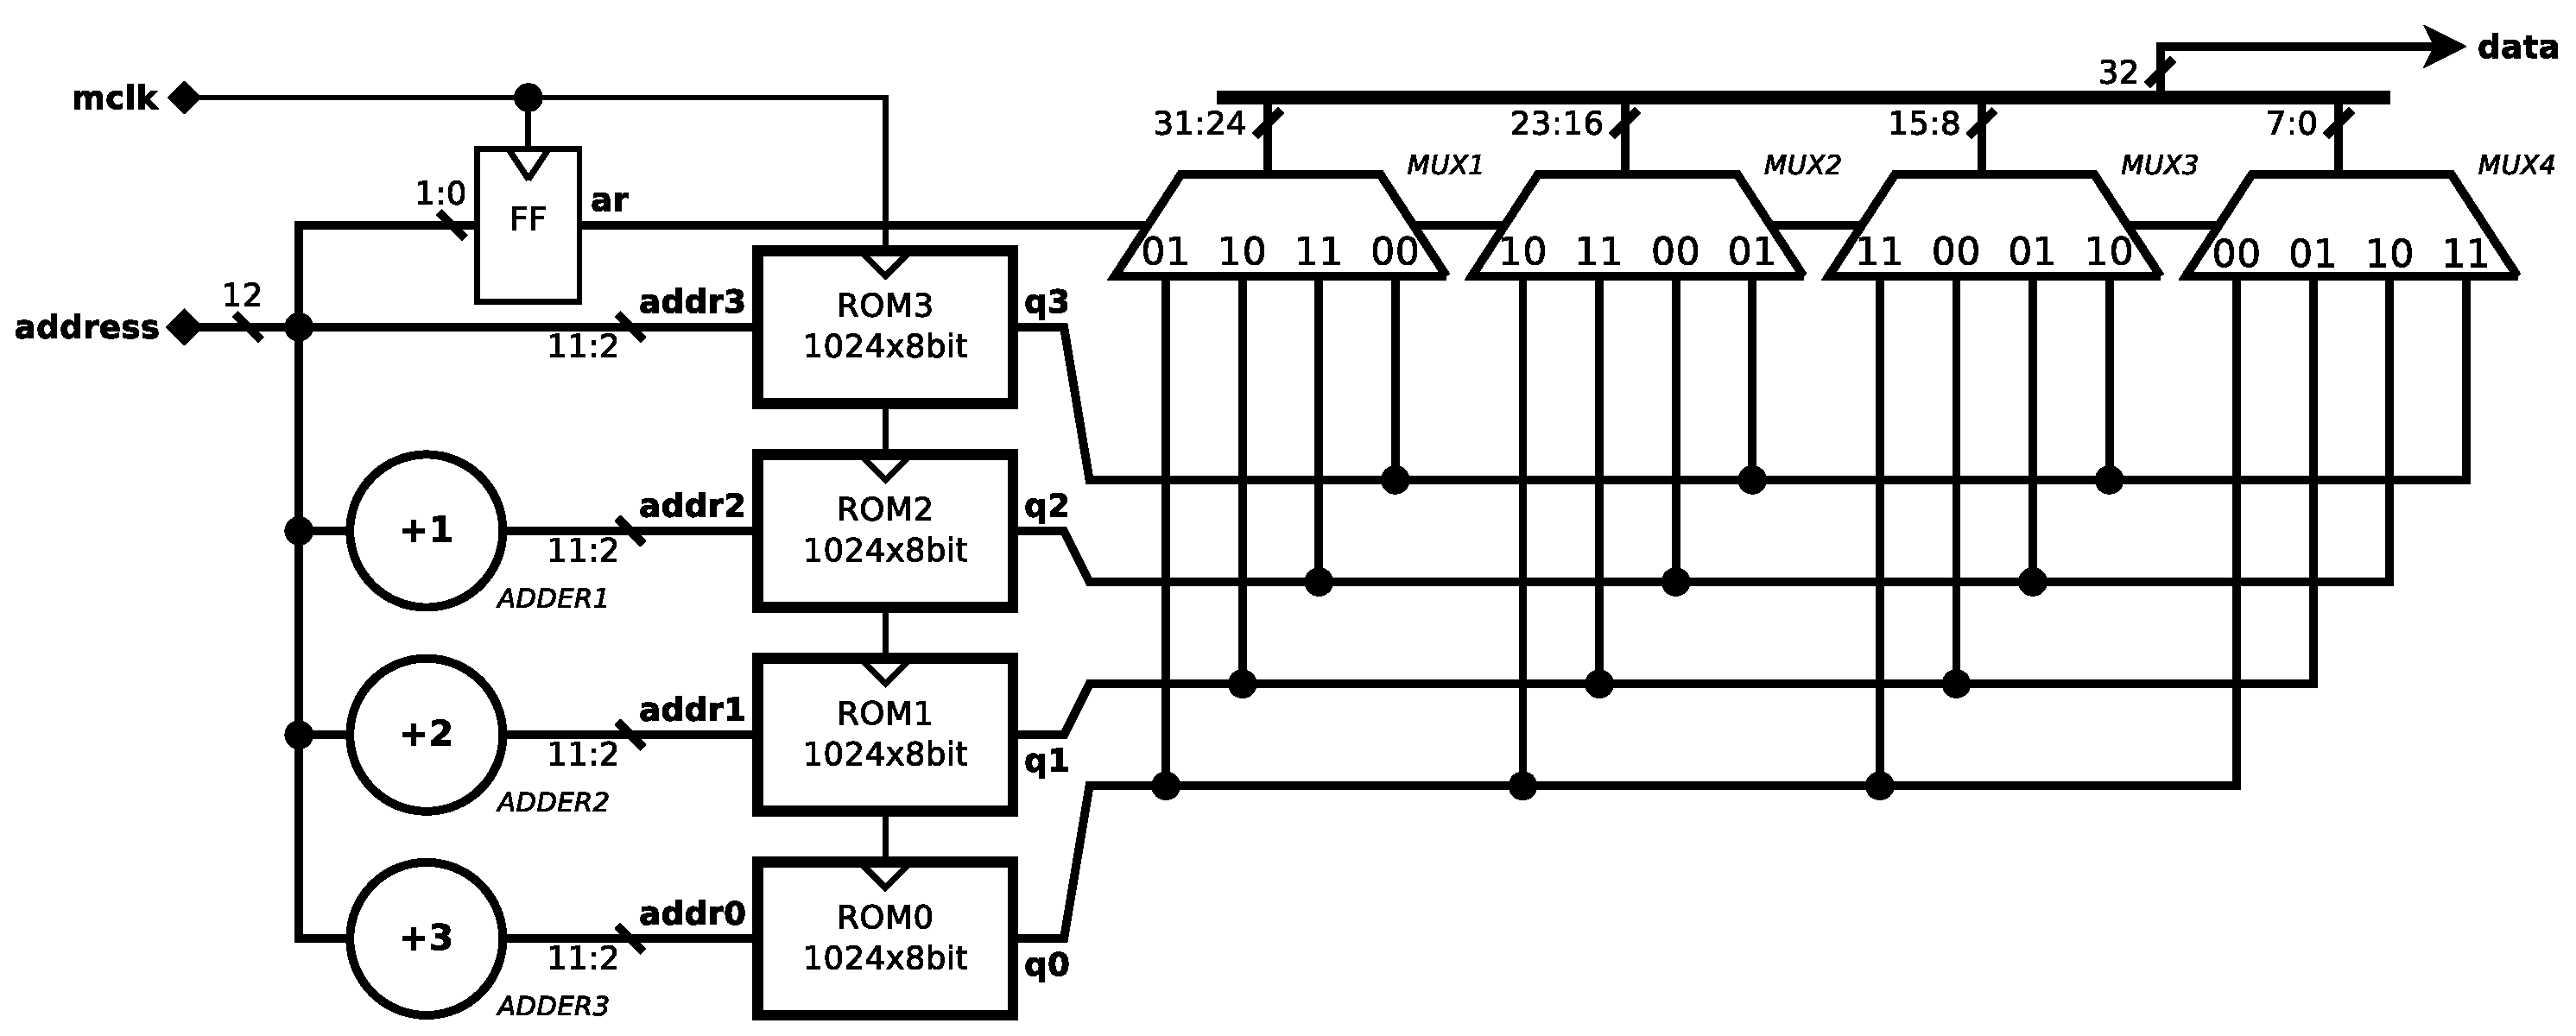
\includegraphics[width=\linewidth]{../resources/risc_mem.eps}
	\caption{Digital diagram of RISC sliced ROM memory logic}
	\label{fig:risc_mem}
\end{figure*}

\subsubsection{RISC Program Memory}
In order to allow a dynamic instruction size from one to four bytes, a special memory arrangement is made. A system was re-
quired to access a word (8bits) from memory and next three words, meaning that memory cannot simply be packed to four word segments. To achieve desired functionality, four ROM blocks been utilised, each containing one fourth of sliced original data. Input address is offset by adders \textit{ADDER1-3} and further divided by value four, which is done by removing two least significant bits at \textbf{addr0-3}. 
Before concatenating output of each ROM block into final four bytes, ROM outputs \textbf{q0-3} are rearranged depending on \textbf{ar} signal. Note that \textit{MUX1-4} each input is different, this may be better visualised with Verilog code in listing \ref{code:rom_switch}.


\begin{blockpage}
\begin{lstlisting}[frame=single, language=Verilog, caption={RISC sliced ROM memory multiplexer arrangement Verilog code}, emph={ar, data}, label=code:rom_switch]
case(ar)
  2'b00: data={q3,q2,q1,q0};
  2'b01: data={q0,q3,q2,q1};
  2'b10: data={q1,q0,q3,q2};
  2'b11: data={q2,q1,q0,q3};
endcase
\end{lstlisting}
\end{blockpage}

\subsubsection{OISC Program Memory}\label{subsec:oisc_mem}
OISC instructions are fixed 13 bits, this non-standard memory word size causes some difficulties. To implement ROM in FPGA, Altera Cyclone IV M9K configurable memory blocks were used. Each blocks has 9kB of memory, each set as 1024x9bit configuration. Combining three these blocks together yields 27bits if readable data in single clock cycle. To store instruction code to such configuration, pairs of instruction machine code sliced into three parts plus one bit for parity check, see figure \ref{fig:oisc_memory_slice}. Circuit extracting each instruction is fairly simple, shown in figure \ref{fig:oisc_mem}.

\begin{figure*}[t]
\begin{gather*}
\overunderbraces{&\br{1}{ROM0}&\br{2}{ROM1}&\br{2}{ROM2}}%
{&
\colorbox{c1}{\scalebox{0.75}{00}}\,
\colorbox{c1}{\scalebox{0.75}{01}}\,
\colorbox{c1}{\scalebox{0.75}{02}}\,
\colorbox{c1}{\scalebox{0.75}{03}}\,
\colorbox{c1}{\scalebox{0.75}{04}}\,
\colorbox{c1}{\scalebox{0.75}{05}}\,
\colorbox{c1}{\scalebox{0.75}{06}}\,
\colorbox{c1}{\scalebox{0.75}{07}}\,
\colorbox{c1}{\scalebox{0.75}{08}}\,&
\colorbox{c1}{\scalebox{0.75}{09}}\,
\colorbox{c1}{\scalebox{0.75}{10}}\,
\colorbox{c1}{\scalebox{0.75}{11}}\,
\colorbox{c1}{\scalebox{0.75}{12}}\,&
\colorbox{c2}{\scalebox{0.75}{13}}\,
\colorbox{c2}{\scalebox{0.75}{14}}\,
\colorbox{c2}{\scalebox{0.75}{15}}\,
\colorbox{c2}{\scalebox{0.75}{16}}\,
\colorbox{c2}{\scalebox{0.75}{17}}\,&
\colorbox{c2}{\scalebox{0.75}{18}}\,
\colorbox{c2}{\scalebox{0.75}{19}}\,
\colorbox{c2}{\scalebox{0.75}{20}}\,
\colorbox{c2}{\scalebox{0.75}{21}}\,
\colorbox{c2}{\scalebox{0.75}{22}}\,
\colorbox{c2}{\scalebox{0.75}{23}}\,
\colorbox{c2}{\scalebox{0.75}{24}}\,
\colorbox{c2}{\scalebox{0.75}{25}}\,&
\colorbox{c3}{\scalebox{0.75}{26}}\,&
}%
{&\br{2}{InstrA}&\br{2}{InstrB}&\br{1}{parity}}
\end{gather*}
\caption{OISC three memory words composition. Number inside box represents bit index.}
\label{fig:oisc_memory_slice}
\end{figure*}

\begin{figure*}[t]
	\centering
	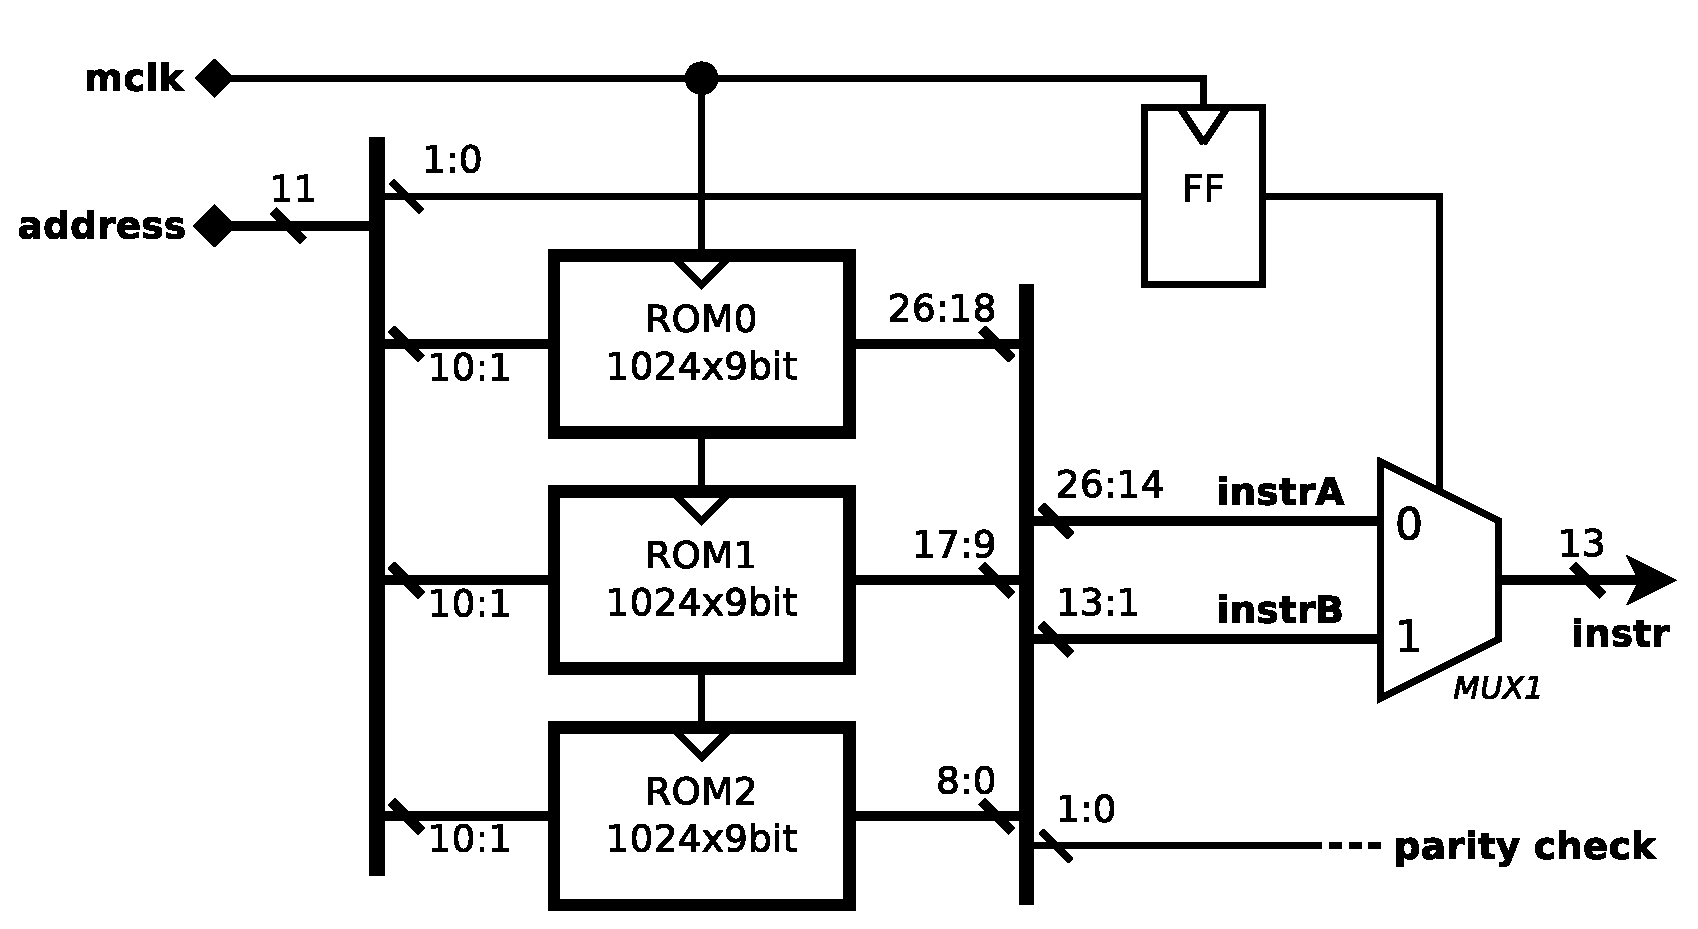
\includegraphics[scale=0.4]{../resources/oisc_mem.eps}
	\caption{Digital diagram of OISC instruction ROM logic}
	\label{fig:oisc_mem}
\end{figure*}

\subsection{Instruction decoding}\label{subsec:imm_values}
This section describes RISC and OISC differences between instruction decoding and immediate value handling.
\subsubsection{RISC IMO} \label{subsec:imo}
Already described in previous section \ref{subsec:memory}, instruction from the memory comes as four bytes. The least significant byte is sent to control block, other three bytes are sent to the immediate override block (IMO) shown in figure \ref{fig:risc_imo}. These three bytes are labelled as \textbf{immr}. 

\begin{figure*}
	\centering
	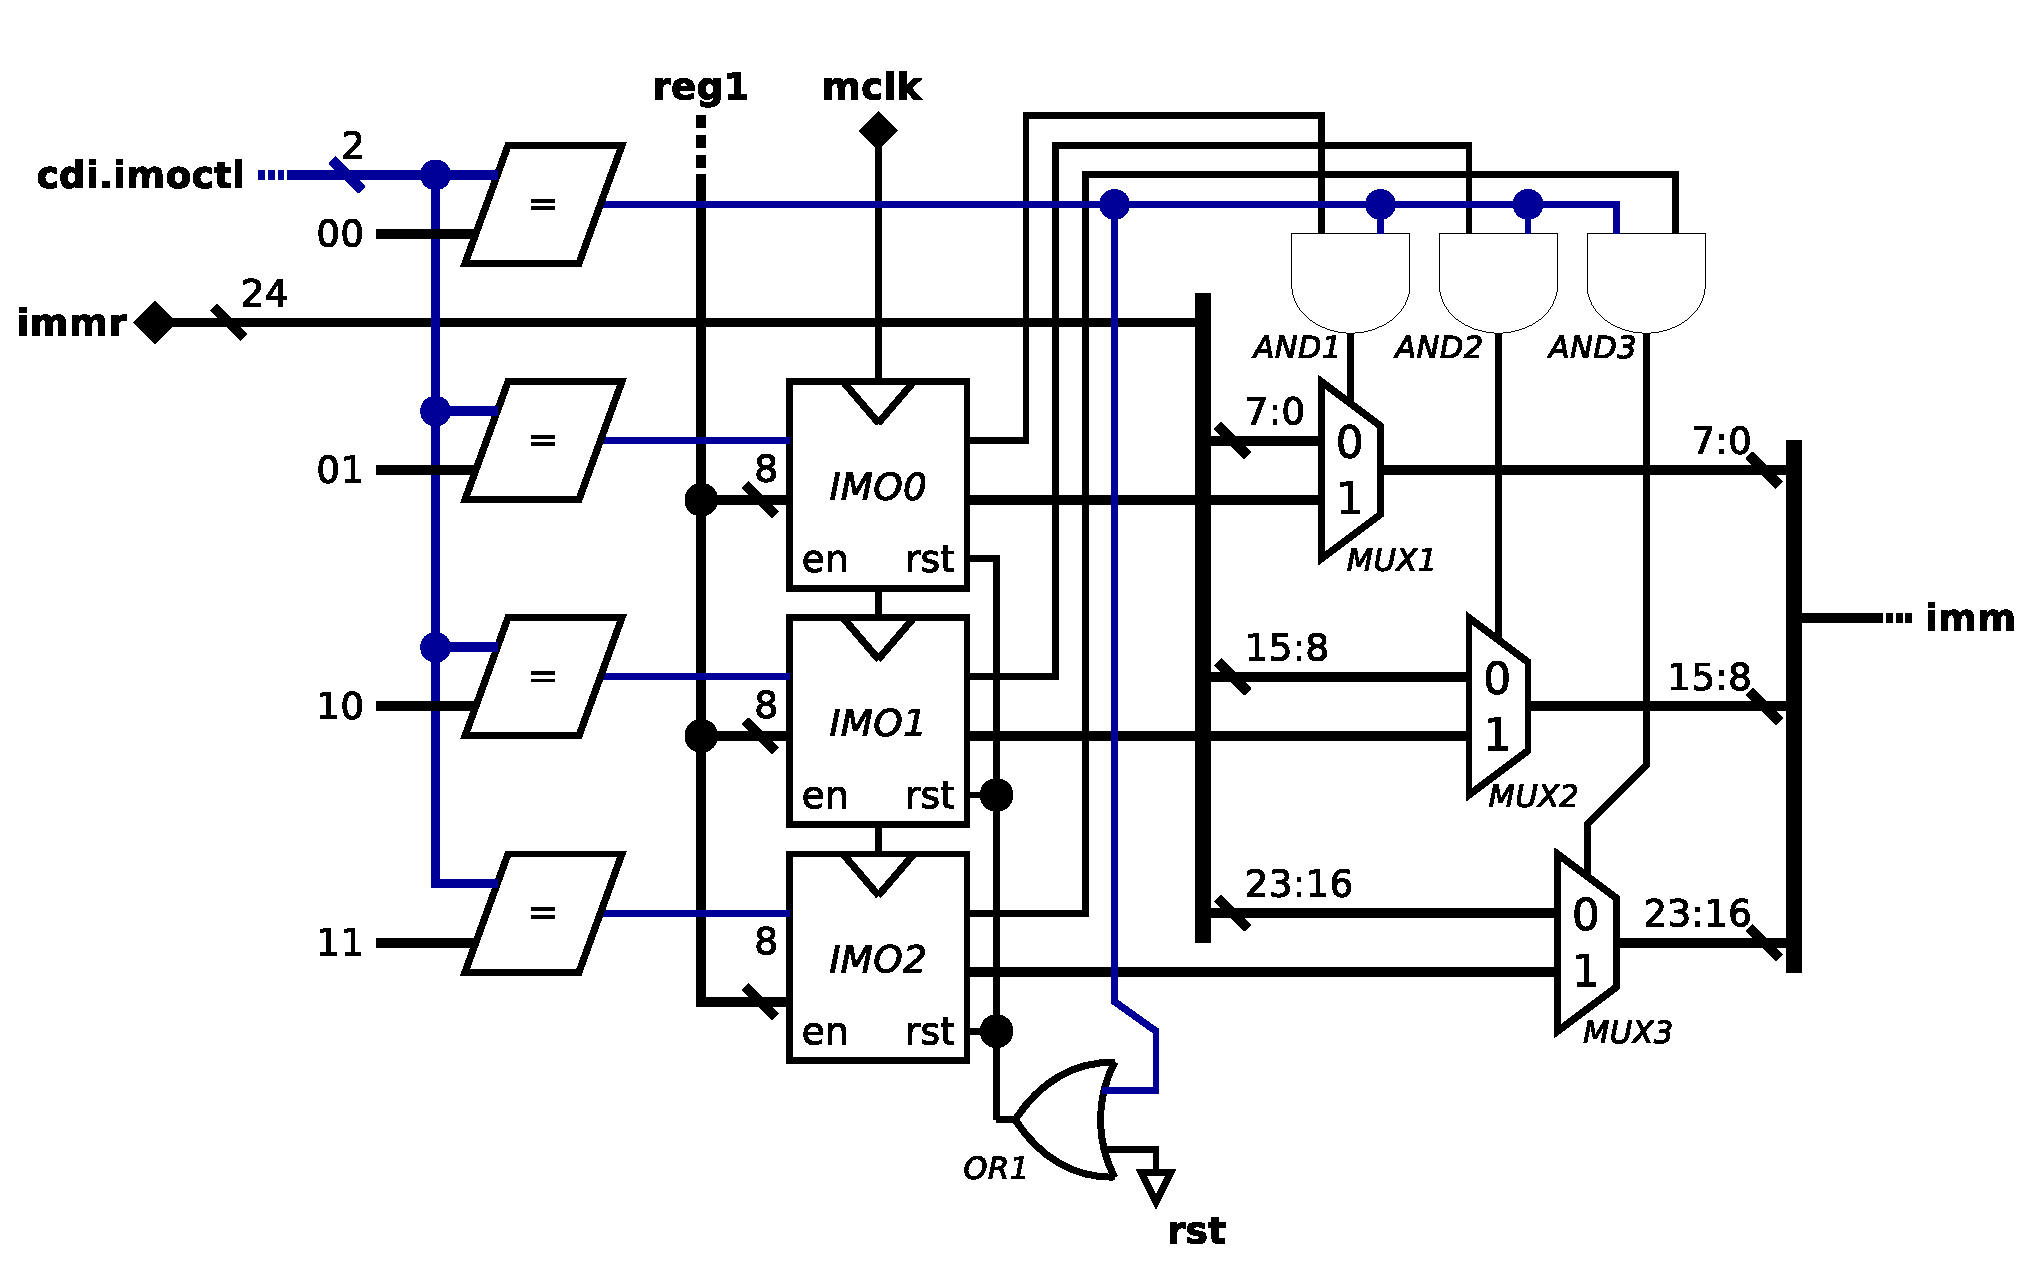
\includegraphics[scale=0.4]{../resources/risc_imo.eps}
	\caption{Digital diagram of RISC immediate override system}
	\label{fig:risc_imo}
\end{figure*}


The IMO block is a solution to change the immediate sent further to the processor with a value from register. This enables dynamically calculated memory pointers, branches that are dependent on a register value or any other function that needs instruction immediate value been replaced by calculated register value. IMO is controlled by control block and \textbf{cdi.imoctl} signal, which is changed by \texttt{CI0}, \texttt{CI1} and \texttt{CI2} instructions. When a signal is \texttt{0h}, this block is transparent connecting \textbf{immr} directly to \textbf{imm}. When any of \texttt{CI} instructions executed, one of IMO register is overwritten by \textit{reg1} value from the register file. In order to override two or three bytes of immediate, \texttt{CI} instructions need to be executed in order. Only for one next instruction after last \texttt{CI} will have immediate bytes changed depending on what are values in \textit{IMO} registers.
\\This circuit has two disadvantages: 
\begin{enumerate}
	\item Overriding immediate bytes takes one or more clock cycles,
	\item At override, \textbf{immr} bytes are ignored therefore they are wasting instruction memory space.
\end{enumerate}
Second point can be resolved by designing a circuit that would subtract the amount of overwritten IMO bytes from \textit{pc\_off} signal (program counter offset that is dependent on i-size value) at the program counter, therefore effectively saving instruction memory space. This solution however, would introduce a complication with the assembler as additional checks would need to be done during assembly compilation to check if IMO instruction are used.

\subsubsection{OISC Instruction decoding}
OISC immediate value is set in instruction decoder shown in figure \ref{fig:oisc_decoder}. Decoder operation is simple - instruction machine code is split into three parts as described in \ref{fig:oisc_machinecode}. If instruction source address value is \texttt{00h}, it connects data bus with constant zero value via \textit{MUX2}. If immediate flag is set, source address value is set to \texttt{00h} in order to make sure no other buffer source connects to data bus. Instruction source address then is connected to databus via \textit{MUX2} and \textit{BUF1}. 

\begin{figure*}
	\centering
	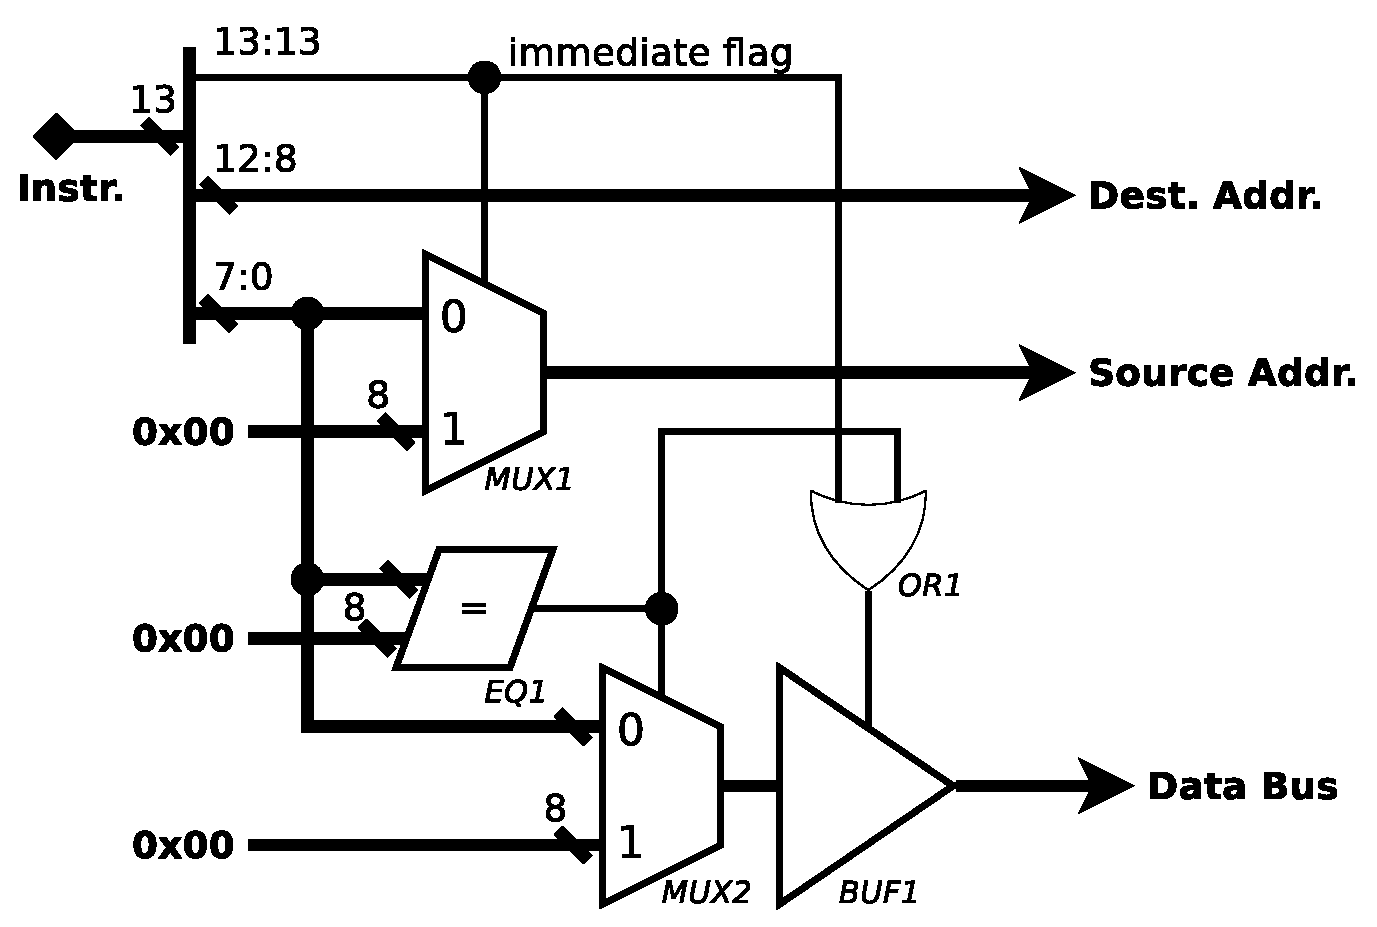
\includegraphics[scale=0.4]{../resources/oisc_decoder.eps}
	\caption{Digital diagram of OISC instruction decoder}
	\label{fig:oisc_decoder}
\end{figure*}

\subsection{Assembly}\label{subsec:assembly}
There are two steps between the assembly code and its execution on a processor. First, it needs to be converted into a binary machine code. Secondly, binary data needs to be sliced to different parts described in section \ref{subsec:memory}. These slices also need to be converted into appropriate formats, different for simulation, HDL synthesis and direct memory flashing. 

A universal assembler was implemented using python for both processors. The flowchart in figure \ref{fig:assembler} represents general structure of assembler process. It splits assembly file into three parts — sections, definitions and macros. Definitions are keywords mapped to values which are saved in a global label dictionary. Macros are a chunk of assembly code and are used as templates. 

There are only two sections implemented in assembler - \texttt{.text} and \texttt{.data}. Section \texttt{.text} contains all machine instructions which will be stored in program ROM memory. Section \texttt{.data} is used for global and static data, and it will be written into RAM memory. This section is used to store values such as strings and uninitialised data structures. These values are accessed with labels which correspond to RAM memory location. 

Section \texttt{.text} code is processed line by line. Each line may have label and an instruction or macro name following with argument values. If line contains a label, it is stored into global label dictionary with current line program address as a value. If line has a macro, line is replaces by macro code. Otherwise, instruction name is decoded and stored in an instruction list with original arguments.

After all instruction lines are completed, each stored instruction arguments are processed, labels are replaced with binary values, any other processing is done such as addition by constant, byte selection, etc. Completed list is then saved as a raw binary. Similarly, \texttt{.data} section labels also replaced and it is saved as binary data.

\begin{colfigure}
	\centering
	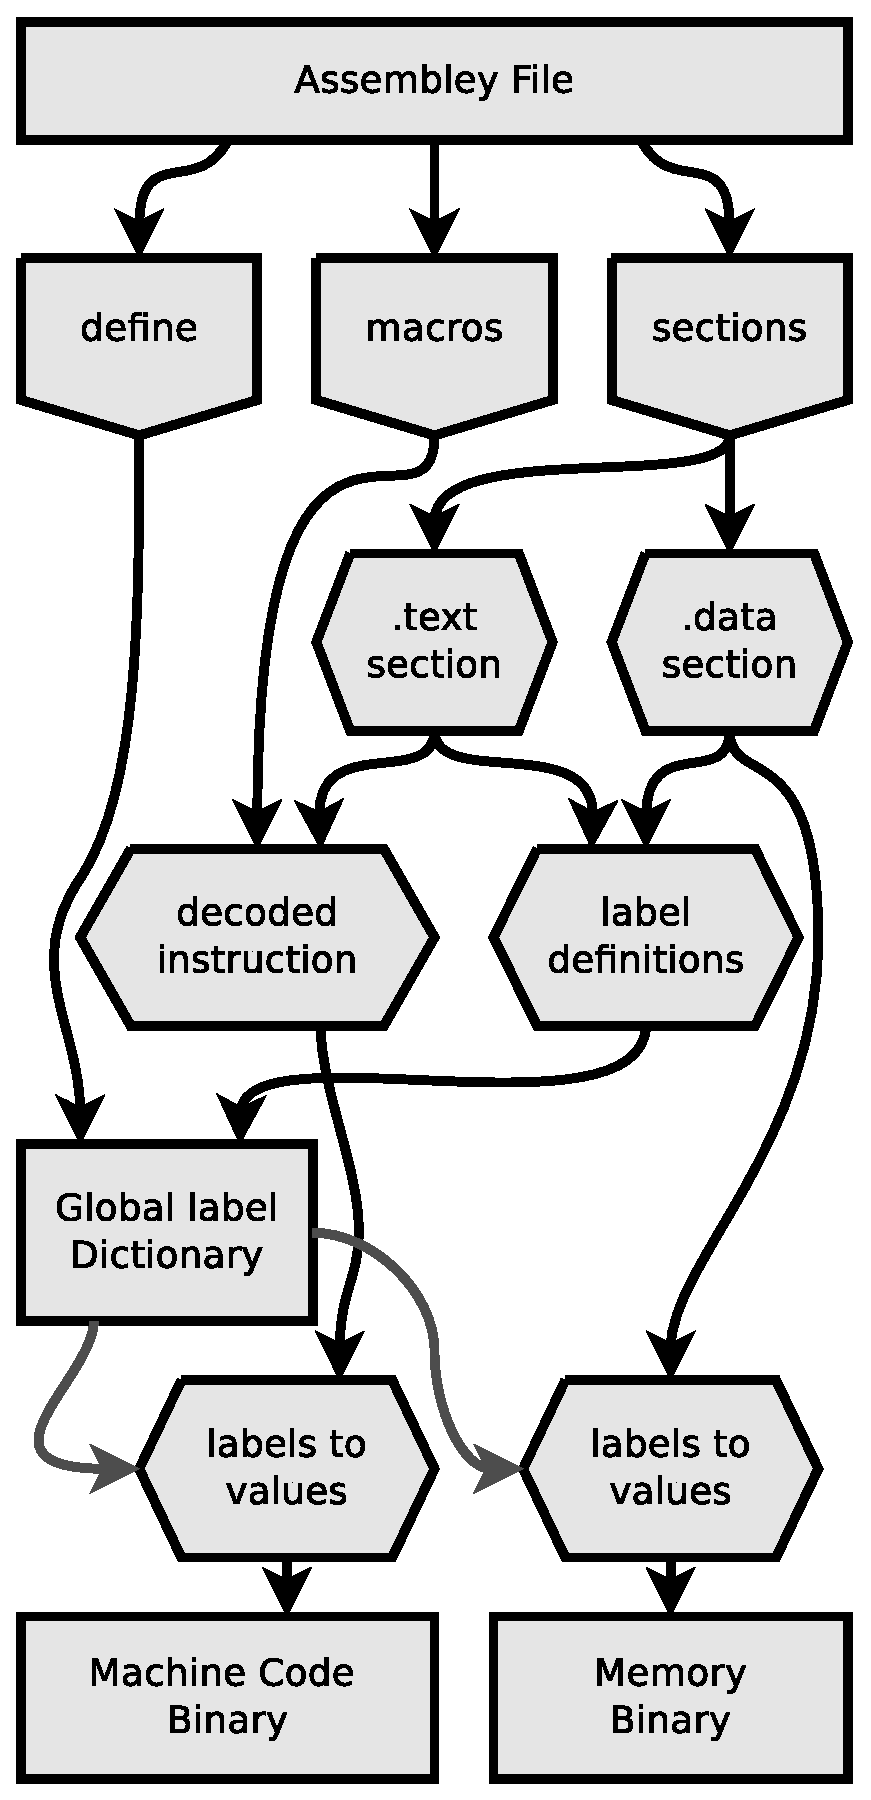
\includegraphics[scale=0.4]{../resources/assembler.eps}
	\captionof{figure}{Flow chart of assember converting assembly code into machine code and memory binary.}
	\label{fig:assembler}
\end{colfigure}

\subsection{System setup}\label{subsec:setup}
This section will describe how the system is set up.

Processors are implemented on Terasic DE0-Nano board that use Altera Cyclone IV, EP4CE22P17C6 FPGA, which is manufactured using $60nm$ fabrication technology.
The FPGA has embedded memory structure consisting of M9K memory blocks columns mentioned in Subsection \ref{subsec:oisc_mem}. These memory structures were used to implement processors RAM and ROM memories. Board also has 32MB SDRAM chip, which initially was intended to be used. This set design criteria to have 24bit address space. However, M9K memory was used instead for flexibility and simplicity. 

Thas FPGA has also an embedded phase-locked loop (PLL) stucture that is used to change 50MHz input that is generated by on-board crystal to other frequencies. 

DE0-Nano board has an integrated JTAG port that is used to upload synthesised code and control additional debugging tools. Quartus has a "Signal Tap Logic Analyzer" tool that allow setup probes and sources within FPGA logic and control them via JTAG. Another "In-System Memory Content Editor" tool allows read and modify M9K memory which enables quick machine code uploading to the processor on FPGA, without need to resynthesise HDL code. This also allow reading RAM content enabling easier program debugging. 

All Quartus functions can be accessed via TCL script. This lead to constructing Makefile which allow quick build operations. Quratus signal and memory tools were used to write a small program with Python and Curses library to read and change internal processor state which allowed easy debugging while writing the programs. 


